The \ac{KVS} is designed for multi-core architectures and relies on both
volatile and non-volatile memory attached to the system memory interface. In
order to take advantage of both types of memory, the \ac{KVS} is designed as a
two-level store which only updates \ac{NVRAM} when a transaction commits.
Consistency across crashes is ensured with existing hardware primitives and
upcoming platform features. Concurrent transactions are controlled by a
serializable variant of \ac{SI}. Background on these design decisions is given
below.

Designing a runtime-critical software such as databases not only involves
knowledge about expected workloads but also about the underlying computing
device. While workloads have been discussed earlier, this section describes the
system architecture of the intended \ac{KVS}.

\subsubsection{Concurrency}

The \ac{KVS} is designed for a single-node architecture. Even though distributed
databases are fairly common, there seems to be no apparent reason for them to
reveal any more insight on leveraging \ac{NVRAM} for concurrency. Also
distributed systems involve much more complex mechanisms such as consensus among
distributed transactions, all of which are beyond the scope of this work.
However, future work should investigate whether the conclusions of this work
also hold for distributed databases.

In order to achieve scalable transaction throughput through concurrency, the
target system is a multi-core architecture. That means, the system features one
or more processors with multiple cores, where each core may support multiple
hardware threads. On such a system, each transaction is executed in the context
of a thread which is scheduled and assigned to a processor core by the operating
system. Processors usually coordinate their work by communicating via some form
of chip interconnect. In order to preserve generality, this work makes no
assumptions concerning the nature of such interconnect networks.

% \begin{figure}[!ht]
\begin{figure}
    \centering
    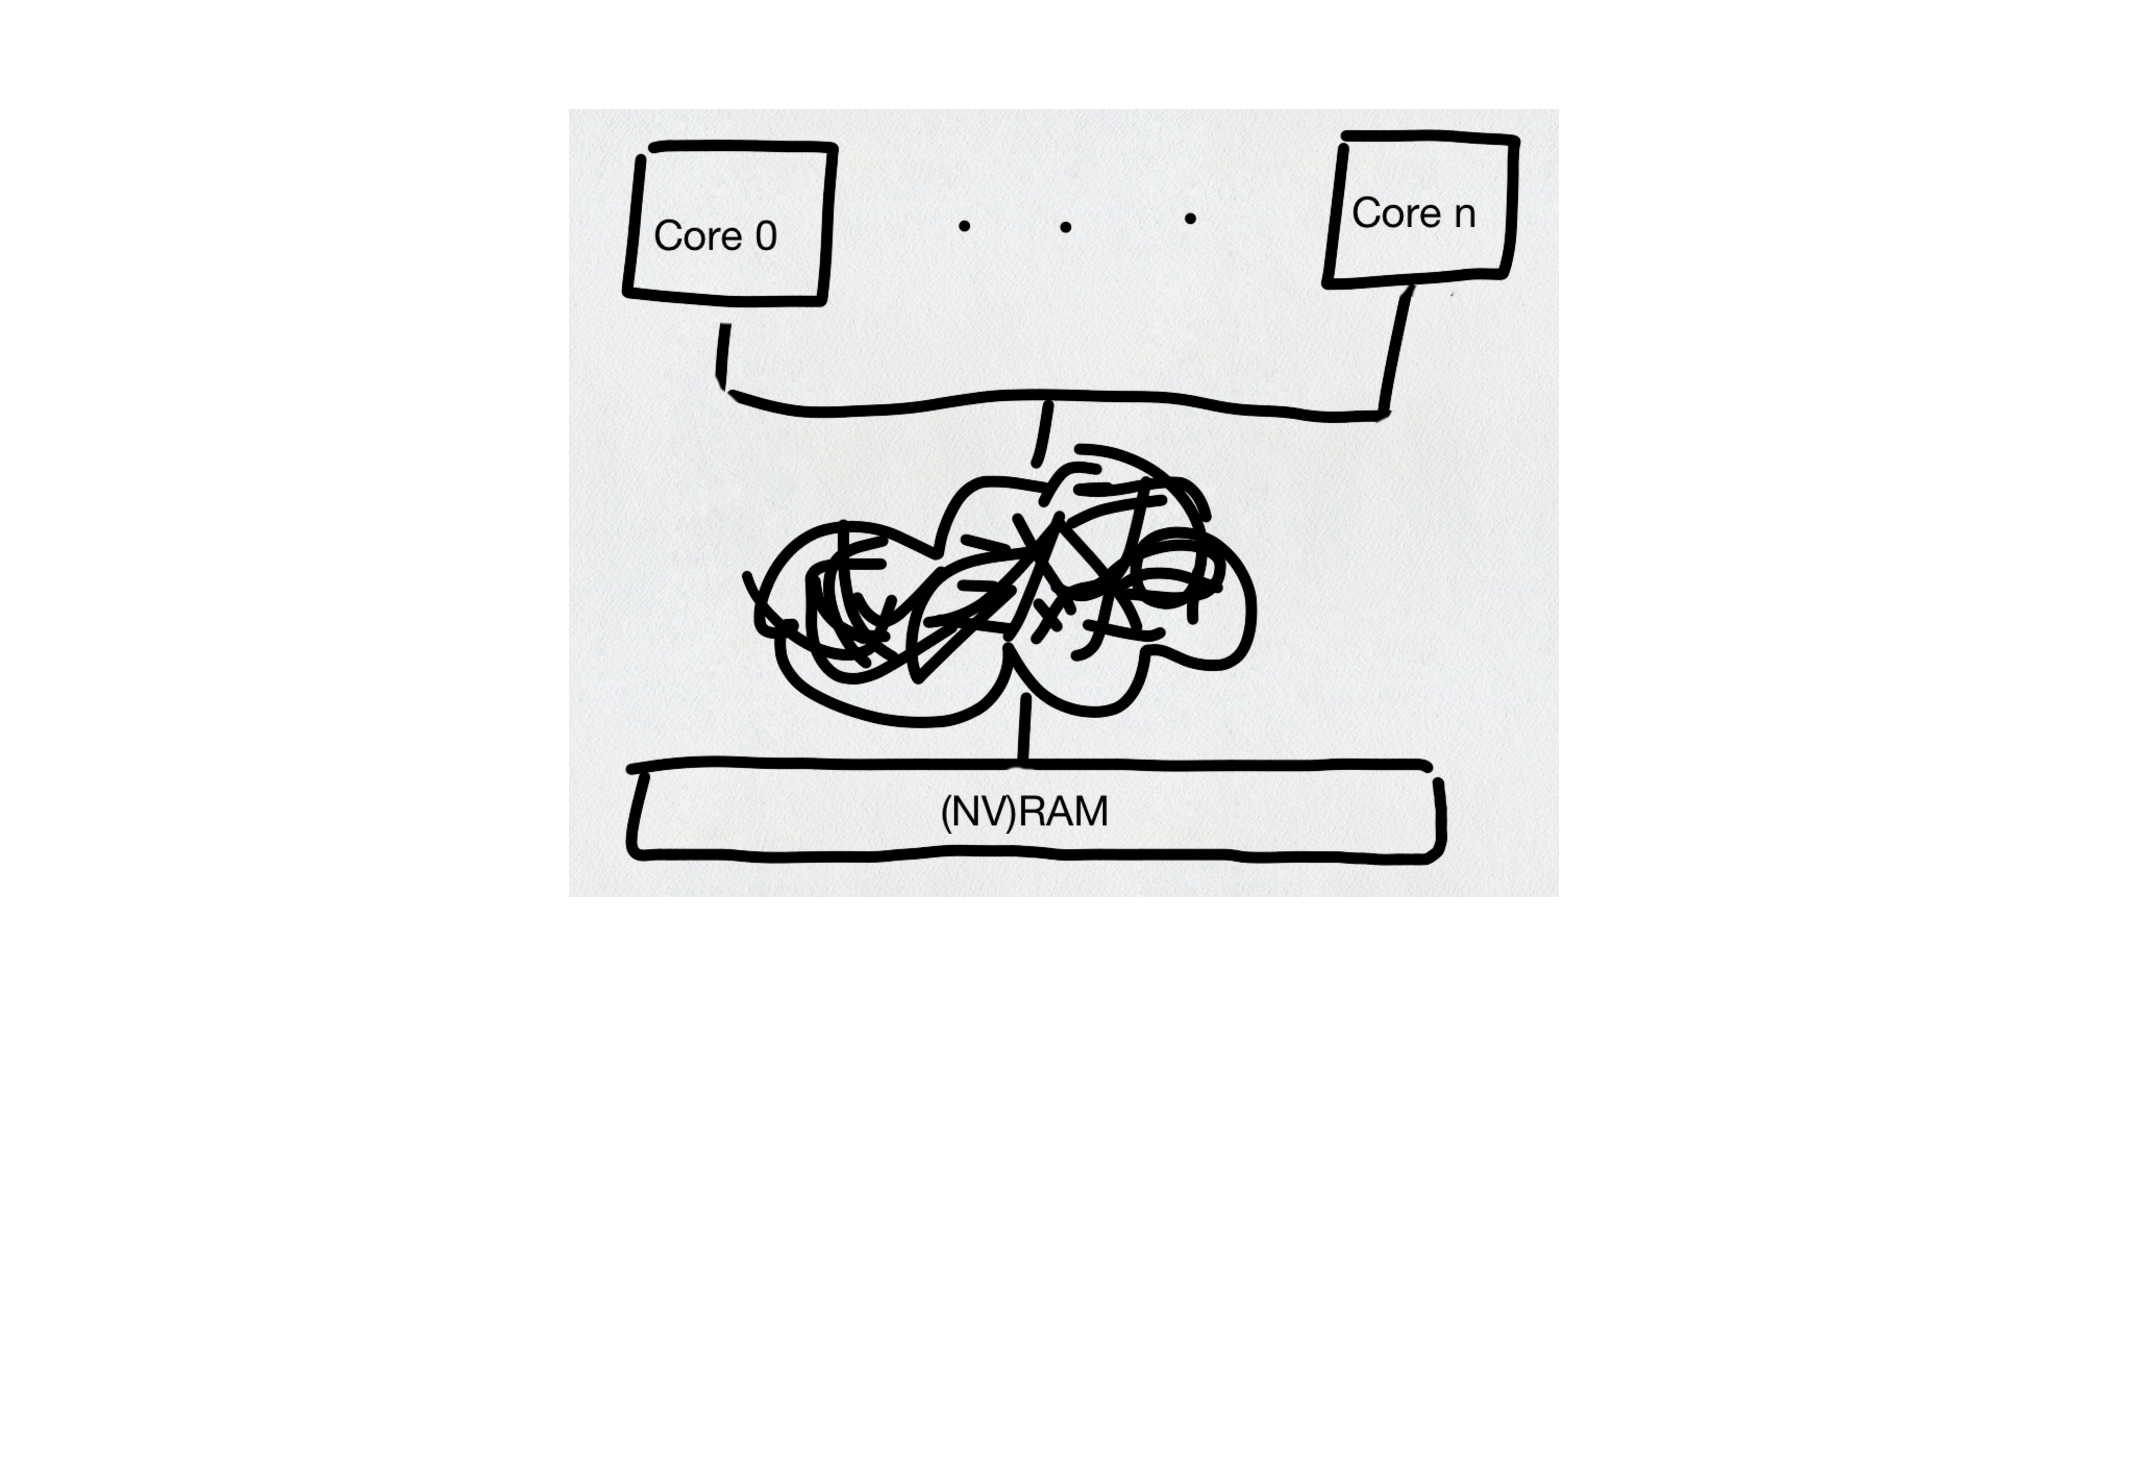
\includegraphics[scale=0.5]{figures/drafts/concept-sys-cpu.pdf}
    \caption{}
    \label{fig:concept-sys-cpu}
\end{figure}

\subsubsection{Memory Architecture}

Recent research shows that on traditional hardware it is advisable to continue
integrating volatile \ac{RAM} together with \ac{NVRAM}. The reason is that not
all data is meant to be durable which is especially true for \ac{NVRAM} where
crash consistency is linked with considerable overhead. Manufacturing \ac{NVRAM}
is still challenging, especially in terms of access latency and endurance, but
it is expected that these issues will be resolved in the near future. Therefore,
in an effort to combine the benefits of both technologies, the memory subsystem
is required to feature both volatile \ac{RAM} and \ac{NVRAM}. In accordance with
recent research it is assumed that both kinds of memory can be accessed through
the same memory interface. This work assumes a shared memory architecture. That
is, processors may have one or more private cache levels but main memory is
accessible to all processors. Conceptually, cache coherence is not required but
has the advantage that less effort is spent on coordinating concurrent access to
shared data.

The \ac{KVS} is designed to exclusively reside in main memory. All data that is
not required across restarts is stored in volatile \ac{RAM}, whereas all other
data are stored in \ac{NVRAM}. Multiple recent works have demonstrated that
\ac{NVRAM} can be used to build \ac{MMDB} without conventional non-volatile
storage such as hard drives. As a result, ensuring recovery, which has always
been an inherent bottleneck of \ac{MMDB}, can be eliminated. In addition,
near-instantaneous restarts become feasible. As a consequence, conventional
storage is not part of the concept for this \ac{KVS}. While such components may
very well be present in a system, they are never used to store any data of the
\ac{KVS} other than its binaries. This way, data access incurs no I/O and
restarts do not have to fetch data from slower storage devices. In return,
candidate systems must provide sufficient \ac{NVRAM} capacity to hold the entire
database.

% \begin{figure}[!ht]
\begin{figure}
    \centering
    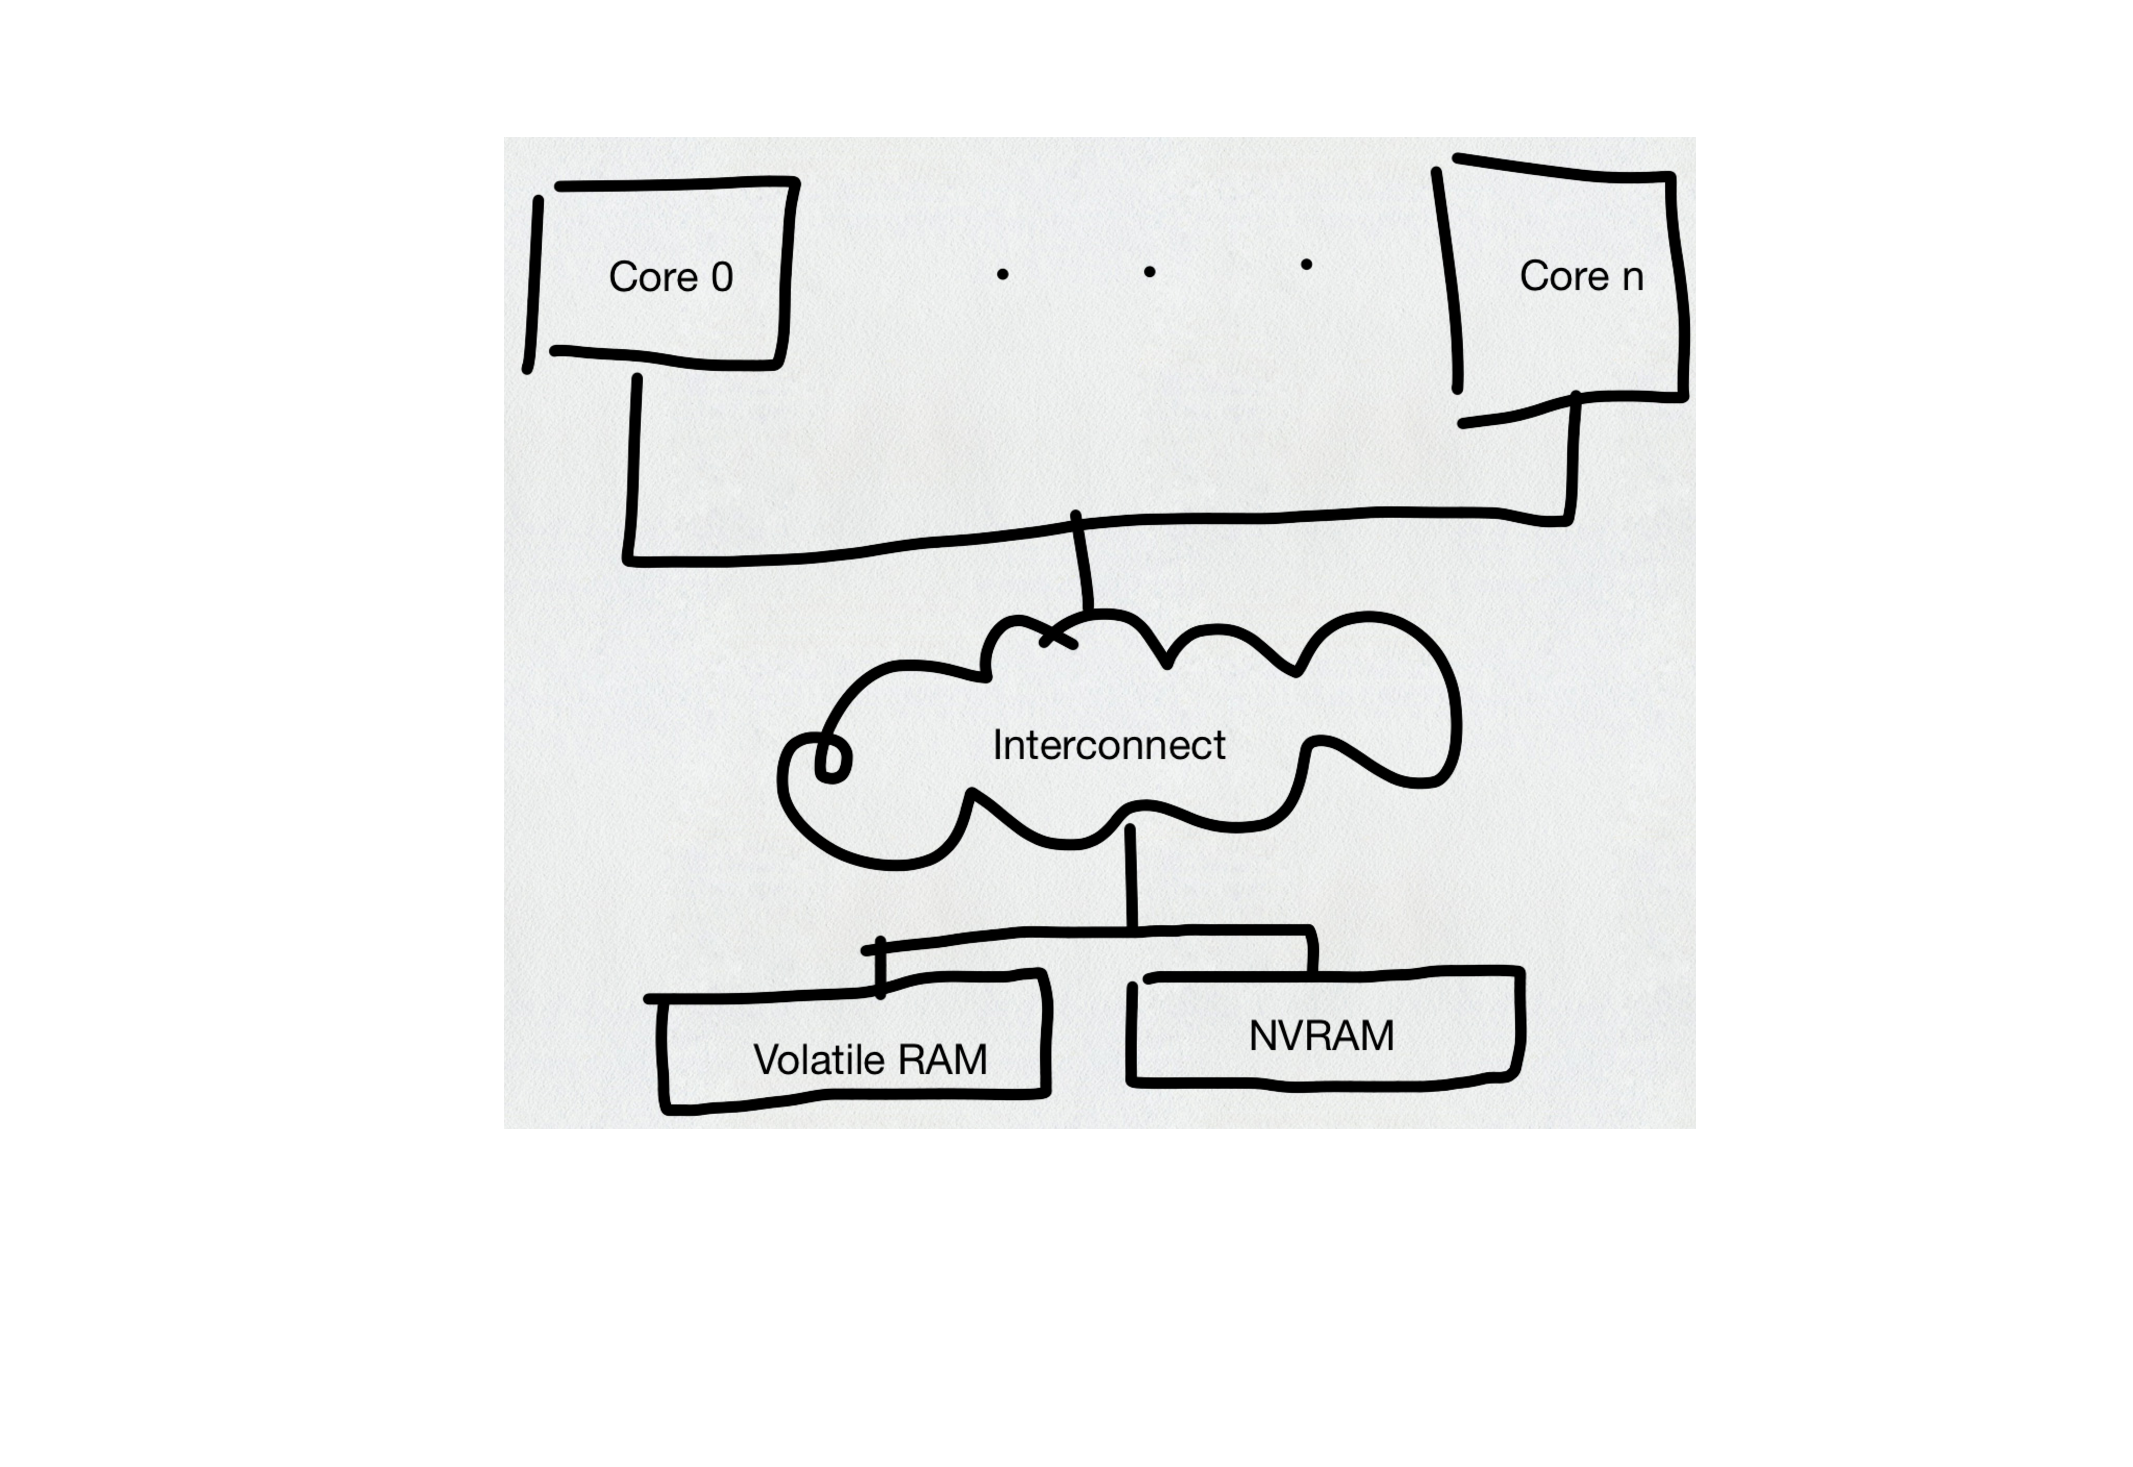
\includegraphics[scale=0.5]{figures/drafts/concept-sys-mem.pdf}
    \caption{}
    \label{fig:concept-sys-mem}
\end{figure}

A disadvantage of this approach is that the size of the database is bounded by
the amount of available \ac{NVRAM}. In contrast, \ac{MMDB} usually allow for
larger data sets by keeping frequently used data in memory, while others are
moved to slower mass storage media. However, main memory capacities have been
steadily growing and \ac{NVRAM} capacities are projected to have at least twice
the capacity of \ac{DRAM}. Another drawback is recoverability in case of device
failures. Mass storage not only scales better in terms of capacity, but it also
supports redundancy through \ac{RAID}, for instance. With \ac{NVRAM}, both
capacity and scalability are lower, so employing information redundancy may be
prohibitively expensive. Without such measures of fault tolerance, however, a
single failed \ac{NVRAM} module may lead to permanent data loss. This issue is
not tackled in this thesis and is therefore left for future work.
